
LLVM后端的任务是从LLVM IR创建机器指令,这个过程叫做指令选择或指令降级。出于尽可能地自动化这个任务的想法,LLVM开发人员发明了TableGen语言来捕获目标描述的所有细节。在深入学习指令选择算法之前,我们先来看看这种语言。\par

\hspace*{\fill} \par %插入空行
\textbf{用TableGen语言指定目标}

机器指令有很多属性:汇编程序和反汇编程序使用的助记符、在内存中表示指令的位模式、输入和输出操作数,等等。LLVM开发人员决定在一个地方捕获所有这些信息,即目标描述。一种新的语言,TableGen语言,就是为此目的而发明的。其想法是使用代码生成器从目标描述创建各种源片段,然后可以在不同的工具中使用这些片段。目标描述存储在使用.td文件中。\par

原则上,TableGen语言非常简单,您所能做的就是定义记录。一个记录有唯一的名称,包含一个值列表和一个超类列表。定义是一个所有值的记录,而类是一个可以有未定义值的记录。类的主要目的是有一个抽象记录,可以用来构建其他抽象或具体的记录。例如,Register类定义了一个寄存器的公共属性,则可以为寄存器R0定义一个具体的记录:\par

\begin{lstlisting}[caption={}]
class Register {
	string name;
}

def R0 : Register {
	let name = "R0";
	string altName = "$0";
}
\end{lstlisting}

使用let关键字覆盖一个值。\par

TableGen语言有很多语法糖,可以使处理记录更容易。一个类可以有一个模板实参,例如:\par

\begin{lstlisting}[caption={}]
class Register<string n> {
	string name = n;
}

def R0 : Register<"R0"> {
	string altName = "$0";
}
\end{lstlisting}

TableGen语言是静态类型的,您必须指定每个值的类型。一些受支持的类型如下:\par

\begin{itemize}
\item bit: 一个位
\item int: 64位整数值
\item bits<n>: 一种由n位组成的整数类型
\item string: 一个字符串
\item list<t>: 类型为t的元素列表
\item dag: 有向无环图(DAG:由指令选择使用)
\end{itemize}

类的名称也可以用作类型。例如,list<register>指定Register类的元素列表。\par

该语言允许使用include关键字包含其他文件。对于条件编译,支持预处理指令\#define、\#ifdef和\#ifndef。\par

LLVM中的TableGen库可以解析用TableGen语言编写的文件,并创建记录的内存表示。您可以使用这个库创建自己的生成器。\par

LLVM自带了自己的生成工具LLVM-tblgen和一些.td文件。后端目标描述包括llvm/target/\allowbreak target.td文件。该文件定义诸如Register、Target或Processor等类。llvm-tblgen工具了解这些类,并从定义的记录中生成C++代码。\par

以MIPS后端为例来看看。目标描述在Mips.td中,文件位于llvm/lib/Target/Mips文件夹,该文件包含Target.td文件。它还定义了目标特性,例如:\par

\begin{tcolorbox}[colback=white,colframe=black]
def FeatureMips64r2 \\
\hspace*{0.5cm}: SubtargetFeature<"mips64r2", "MipsArchVersion",  \\
\hspace*{4cm}"Mips64r2", "Mips64r2 ISA Support", \\
\hspace*{4cm}[FeatureMips64, FeatureMips32r2]>;
\end{tcolorbox}

这些特性可以用来定义CPU模型,例如:\par

\begin{tcolorbox}[colback=white,colframe=black]
def : Proc<"mips64r2", [FeatureMips64r2]>;
\end{tcolorbox}

还包括定义寄存器、指令、调度模型等的其他文件。\par

llvm-tblgen工具可以显示此目标描述定义的记录。如果在build目录下,下面的命令会将记录打印到控制台:\par

\begin{tcolorbox}[colback=white,colframe=black]
\$ bin/llvm-tblgen $\setminus$ \\
\hspace*{0.5cm}-I../llvm-project/llvm/lib/Target/Mips/ $\setminus$ \\
\hspace*{0.5cm}-I../llvm-project/llvm/include $\setminus$ \\
\hspace*{0.5cm}../llvm-project/llvm/lib/Target/Mips/Mips.td
\end{tcolorbox}

与Clang一样,-I选项在包含文件时添加一个要搜索的目录。查看记录对调试有帮助。这个工具的真正目的是从记录中生成C++代码。例如,使用-gen-subtarget选项,解析llc的-mcpu=和-mtarget=所需的数据将发送到控制台:\par

\begin{tcolorbox}[colback=white,colframe=black]
\$ bin/llvm-tblgen $\setminus$ \\
\hspace*{0.5cm}-I../llvm-project/llvm/lib/Target/Mips/ $\setminus$ \\
\hspace*{0.5cm}-I../llvm-project/llvm/include $\setminus$ \\
\hspace*{0.5cm}../llvm-project/llvm/lib/Target/Mips/Mips.td $\setminus$ \\
\hspace*{0.5cm}-gen-subtarget
\end{tcolorbox}

将该命令生成的代码保存在一个文件中,并探索如何在生成的代码中使用该特性和CPU !\par

指令的编码通常遵循一些模式。因此,将指令的定义分为定义位编码的类和指令的具体定义类。MIPS指令编码在llvm/Target/Mips/MipsInstrFormats.td文件中。让我们来看看ADD\underline{~}FM格式的定义:\par

\begin{tcolorbox}[colback=white,colframe=black]
class ADD\underline{~}FM<bits<6> op, bits<6> funct> : StdArch \{ \\
\hspace*{0.5cm}	bits<5> rd; \\
\hspace*{0.5cm}	bits<5> rs; \\
\hspace*{0.5cm}	bits<5> rt; \\
\\
\hspace*{0.5cm}	bits<32> Inst; \\
\\
\hspace*{0.5cm}	let Inst{31-26} = op; \\
\hspace*{0.5cm}	let Inst{25-21} = rs; \\
\hspace*{0.5cm}	let Inst{20-16} = rt; \\
\hspace*{0.5cm}	let Inst{15-11} = rd; \\
\hspace*{0.5cm}	let Inst{10-6} = 0; \\
\hspace*{0.5cm}	let Inst{5-0} = funct; \\
\}
\end{tcolorbox}

在记录主体中,定义了几个新的位域:rd、rs等。它们用于覆盖Inst字段的部分,该字段保存指令的位模式。rd、rs和rt位域对指令操作的寄存器进行编码,而op和funct参数表示操作码和函数号。StdArch超类只添加一个字段,声明该格式遵循的编码标准。\par

MIPS目标中的大多数指令编码不指向DAG节点,也不指定汇编助记符。为此定义了一个单独的类。MIPS体系结构中的一个指令是nor指令,它按位计算第一和第二输入寄存器的值,将结果的位倒转,并将结果赋给输出寄存器。该指令有几种变体,下面的LogicNOR类可以避免多次使用相同的定义:\par

\begin{tcolorbox}[colback=white,colframe=black]
class LogicNOR<string opstr, RegisterOperand RO>: \\
\hspace*{0.5cm}InstSE<(outs RO:\$rd), (ins RO:\$rs, RO:\$rt), \\
\hspace*{3cm}!strconcat(opstr, "\t\$rd, \$rs, \$rt"), \\
\hspace*{3cm}[(set RO:\$rd, (not (or RO:\$rs, RO:\$rt)))], \\
\hspace*{3cm}II\underline{~}NOR, FrmR, opstr> \{ \\
\hspace*{0.5cm}let isCommutable = 1; \\
\}
\end{tcolorbox}

哇,记录这个简单的概念现在看起来很复杂。让我们解析一下这个定义:这个类派生自InstSE类,它用于具有标准编码的指令。如果进一步跟踪超类的层次结构,就会看到这个类派生自指令类,指令类是预定义的类,表示目标的一条指令。(outs RO:\$rd)参数将最后一条指令的结果定义为DAG节点。RO部分是指与LogicNOR类同名的参数,表示寄存器操作数,\$rd是要使用的寄存器。在rd字段中,这是以后要放到指令编码中的值。第二个参数定义指令将操作的值。总之,这个类用于在三个寄存器上操作的指令。strconcat(opstr, "$\setminus$t\$rd, \$rs, \$rt")参数汇编指令的文本表示。strconcat操作符是TableGen预定义的函数,用于连接两个字符串。可以在TableGen开发者指南中查找所有预定义的操作符:\url{https://llvm.org/docs/TableGen/ProgRef.html}。\par

记录遵循模式定义,类似于nor指令的文本描述,并描述该指令的计算。模式的第一个元素是操作,后面是用逗号分隔的操作数列表。操作数引用DAG参数中的寄存器名称,并指定LLVM IR值类型。LLVM有一组预定义的操作符,例如add和and,可以在模式中使用。这些操作符属于SDNode类,也可以用作参数。您可以在llvm/Target/TargetSelectionDAG.td中查找预定义的操作符。\par

II\underline{~}NOR参数指定在调度模型中使用的路线类,而FrmR参数是定义来标识这种指令格式的值。最后,opstr助记符传递给超类。这个类的主体非常简单:它只指定nor操作是可交换的,这意味着操作数的顺序可以交换。\par

最后,这个类用于定义一条指令的记录,例如:64位模式下的nor指令:\par

\begin{tcolorbox}[colback=white,colframe=black]
def NOR64 : LogicNOR<"nor", GPR64Opnd>, ADD\underline{~}FM<0, 0x27>,  \\
\hspace*{6cm}GPR\underline{~}64;
\end{tcolorbox}

这是最终的定义,可以通过def关键字识别。它使用LogicNOR类来定义DAG操作数和模式,并使用ADD\underline{~}FM类来指定二进制指令编码。附加的GPR\underline{~}64谓词可以确保该指令仅在64位寄存器上可用。\par

开发人员努力避免多次重复定义,一种常用的方法是使用multiclass类。一个multiclass类可以一次定义多个记录。\par

例如,MIPS CPU的浮点单元可以使用单精度或双精度浮点值进行加法运算。这两条指令的定义非常相似,因此multiclass类定义为一次创建两条指令:\par

\begin{tcolorbox}[colback=white,colframe=black]
multiclass ADDS\underline{~}M<…> \{ \\
\hspace*{1cm}def \underline{~}D32 : ADDS\underline{~}FT<…>, FGR\underline{~}32; \\
\hspace*{1cm}def \underline{~}D64 : ADDS\underline{~}FT<…>, FGR\underline{~}64; \\
\}
\end{tcolorbox}

FT类定义了指令格式,类似于LogicNOR类。FGR\underline{~}32和FGR\underline{~}64谓词在编译时决定可以使用哪条指令。重要的是\underline{~}D32和\underline{~}D64记录的定义,这些是记录的模板。然后用defm关键字定义指令记录:\par

\begin{tcolorbox}[colback=white,colframe=black]
defm FADD : ADDS\underline{~}M<…>;
\end{tcolorbox}

这将同时定义来自多类的两条记录,并将名称FADD\underline{~}D32和FADD\underline{~}D64赋给它们。这是避免代码重复的一种非常强大的方法,它经常用于目标描述,但与其他TableGen特性相结合,可能导致定义模糊。\par

有了目标描述是如何组织的知识,就可以在下一节中探索指令选择。\par

\hspace*{\fill} \par %插入空行
\textbf{指令选择与选择DAG}

LLVM将IR转换为机器指令的标准方法是通过DAG。使用与目标描述中提供的模式匹配的模式,并使用自定义代码,IR指令将转换为机器指令。这种方法并不像听起来那么简单:IR主要是独立于目标的,并且可以包含目标不支持的数据类型。例如,表示单个位的i1类型在大多数目标上不是有效类型。\par

selectionDAG由SDNode类型的节点组成,在llvm/CodeGen/SelectionDAGNodes.h文件中定义。该节点表示的操作称为OpCode,目标独立代码定义在llvm/CodeGen/ISDOpcodes.h文件中。除了操作之外,节点还存储操作数及其生成的值。\par

节点的值和操作数形成数据流依赖关系。控制流依赖由链边表示,链边具有特殊类型MVT::Other。这使得保留具有副作用的指令的顺序成为可能,例如:load指令。\par

使用选择DAG进行指令选择的步骤如下:\par

\begin{enumerate}
\item 构建DAG。
\item 优化DAG。
\item 检查DAG中类型的合法性。
\item 优化DAG。
\item 检查DAG中操作的合法性。
\item 优化DAG。
\item 选择指令。
\item 指令排序。
\end{enumerate}

让我们检查一下每个步骤对选择DAG所做的更改。\par

\hspace*{\fill} \par %插入空行
\textbf{如何进行指令选择}

可以通过两种不同的方式看到指令选择的工作。如果将-debug-only=isel选项传递给llc工具,则每一步的结果都会以文本格式打印出来。如果需要调查为什么选择机器指令,这会有很大的帮助。例如,运行以下命令查看总和的输出.ll文件来自理解LLVM目标后端结构一节:\par

\begin{tcolorbox}[colback=white,colframe=black]
\$ llc -mtriple=mips-linux-gnu -debug-only=isel < sum.ll
\end{tcolorbox}

这会打印出很多信息。在输出的顶部,您可以看到为输入创建的初始DAG的描述:\par

\begin{tcolorbox}[colback=white,colframe=black]
Initial selection DAG: \%bb.0 'sum:' \\
SelectionDAG has 12 nodes: \\
\hspace*{0.5cm}t0: ch = EntryToken \\
\hspace*{2.5cm}t2: i32,ch = CopyFromReg t0, Register:i32 \%0 \\
\hspace*{2cm}t5: i16 = truncate t2 \\
\hspace*{2.5cm}t4: i32,ch = CopyFromReg t0, Register:i32 \%1 \\
\hspace*{2cm}t6: i16 = truncate t4 \\
\hspace*{1.5cm}t7: i16 = add t5, t6 \\
\hspace*{1cm}t8: i32 = any\underline{~}extend t7 \\
\hspace*{0.5cm}t10: ch,glue = CopyToReg t0, Register:i32 \$v0, t8 \\
\hspace*{0.5cm}t11: ch = MipsISD::Ret t10, Register:i32 \$v0, t10:1 
\end{tcolorbox}

与上一节的MIR输出类似,可以在这里看到CopyFromReg指令,它将ABI使用的寄存器的内容转移到虚拟节点。截断节点是必需的,因为示例使用16位值,但是MIPS体系结构只支持32位值。在16位虚拟寄存器上执行添加操作,并将结果扩展并返回给调用者。上面提到的每个步骤都会打印这个部分。\par

LLVM还可以在Graphviz软件的帮助下生成选择DAG的可视化。如果将–view-dag-combine1-dags选项传递给llc工具,则会打开一个窗口,显示构建的DAG。例如,使用前面的小文件运行llc:\par

\begin{tcolorbox}[colback=white,colframe=black]
\$ llc -mtriple=mips-linux-gnu –view-dag-combine1-dags sum.ll
\end{tcolorbox}

在Windows PC上运行,将会看到DAG:\par

\hspace*{\fill} \par %插入空行
\begin{center}
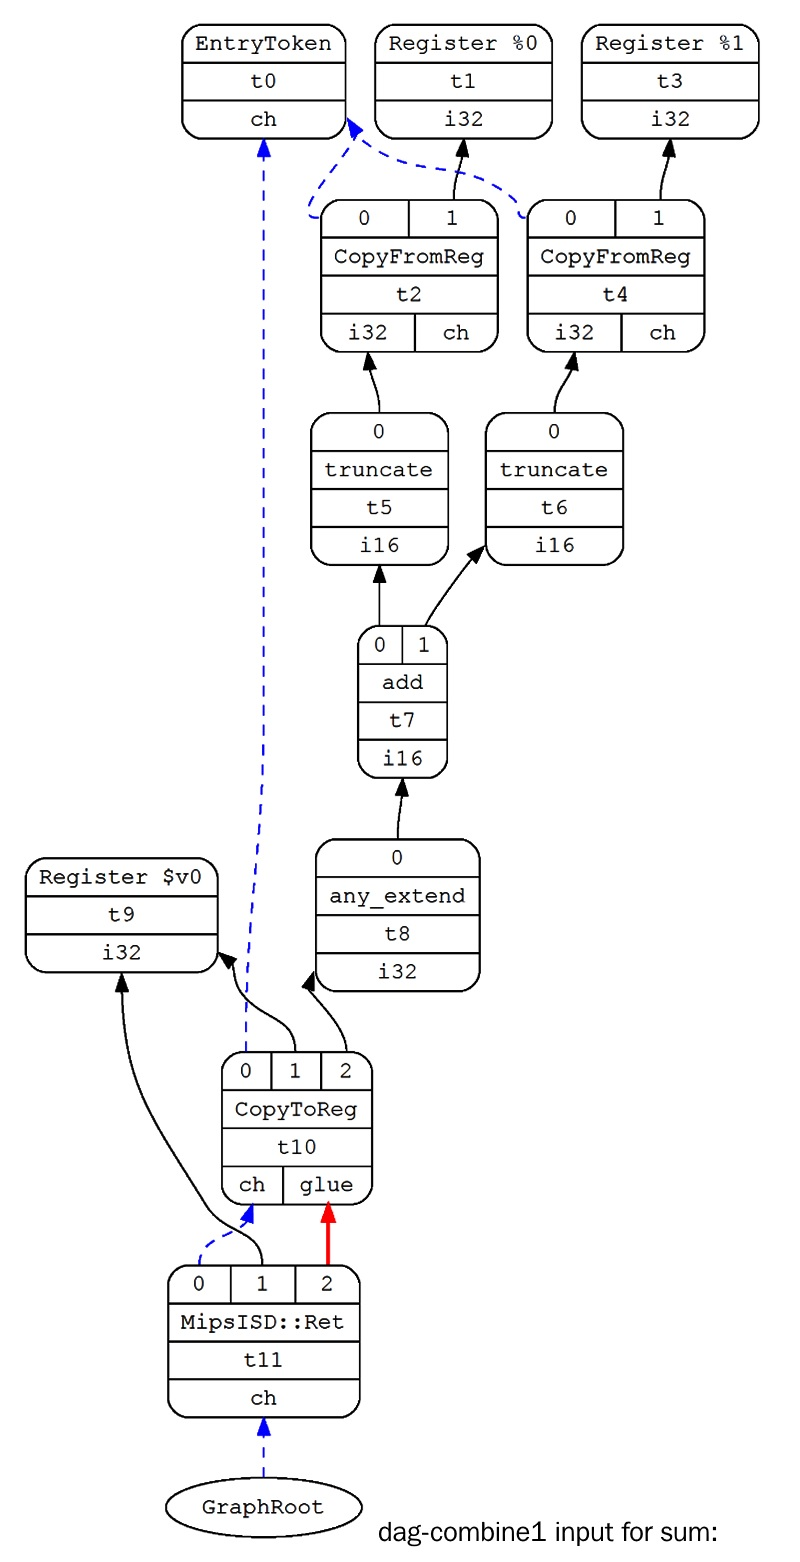
\includegraphics[width=0.55\textwidth]{content/3/chapter9/images/1.jpg}\\
图9.1 – 使用sum.ll构造选择DAG图
\end{center}

一定要比较文本表示和这个图包含相同的信息。EntryToken是DAG的开始,GraphRoot是最后一个节点。控制流的链用蓝色虚线箭头标记,黑色箭头表示数据流,红色箭头将节点粘在一起,防止它们重新排序。即使对于中等大小的函数,图也会变得非常大。它并不比带有-debug-only=isel选项的文本输出更多或其他信息,只是表示的方式更友好。也可以在其他时间点生成图表,例如:\par

\begin{itemize}
\item 添加\verb|--|view-legalize-types-dags选项,在类型合法化之前查看DAG。
\item 添加-view-isel-dags选项以查看指令选择。
\end{itemize}

可以使用\verb|--|help-hidden选项查看所有可用的DAG选项。因为DAG可能会变得很大,而且容易混淆,所以可以使用-filter-view-dags选项将输出限制为一个基本块。\par

\hspace*{\fill} \par %插入空行
\textbf{检查指令选择}

知道了如何形象化DAG,我们现在可以深入到细节。选择DAG是由IR构建的。对于IR中的每个函数,SelectionDAG类的一个实例由SelectionDAGBuilder类填充。不过,在此步骤中没有进行特殊的优化。然而,目标需要提供一些函数来降级调用、参数处理、返回跳转等。为此,目标必须实现targetlower接口。在目标文件夹中,源文件通常在XXXISelLowering.h 和XXXISelLowering.cpp文件中。targetlower接口的实现提供指令过程所需的所有信息,例如:目标上支持哪些数据类型和哪些操作。\par

优化步骤会运行几次。优化器执行简单的优化,例如:在支持这些操作的目标上进行标识重排。这里的基本原理是生成一个清理过的DAG,这里简化了其他步骤。\par

在类型合法化步骤期间,目标上不支持的类型将被支持的类型替换,例如:如果目标本机只支持32位范围的整数,那么较小的值必须通过符号或0扩展名转换为32位。如果一个64位的值不能被这个目标处理,那么这个值必须被分割成一对32位的值。向量类型也以类似的方式处理,vector类型可以使用额外的元素进行扩展,也可以将其分解为几个值。例如,一个有四个值的向量可以分成两个各有两个值的向量。如果拆分过程以单个值结束,则找不到合适的向量,而使用标量类型。有关支持类型的信息是在targetlower接口的特定目标实现中配置的。在类型合法化之后,选择DAG转存文本表示到sum.ll文件中:\par

\begin{tcolorbox}[colback=white,colframe=black]
Optimized type-legalized selection DAG: \%bb.0 'sum:' \\
SelectionDAG has 9 nodes: \\
\hspace*{0.5cm}t0: ch = EntryToken \\
\hspace*{1.5cm}t2: i32,ch = CopyFromReg t0, Register:i32 \%0 \\
\hspace*{1.5cm}t4: i32,ch = CopyFromReg t0, Register:i32 \%1 \\
\hspace*{1cm}t12: i32 = add t2, t4 \\
\hspace*{0.5cm}t10: ch,glue = CopyToReg t0, Register:i32 \$v0, t12 \\
\hspace*{0.5cm}t11: ch = MipsISD::Ret t10, Register:i32 \$v0, t10:1
\end{tcolorbox}

如果与初始构造的DAG进行比较,则这里只使用了32位寄存器。因为本地只支持32位值,所以提升了16位。\par

操作合法化类似于类型合法化。这个步骤是必要的,因为目标不是所有的操作都能支持,或者即使目标本地支持某种类型,也不能对所有操作都有效。例如,并不是所有的目标都有一个针对总体计数的本机指令。在这种情况下,操作被一系列实现功能的操作所取代。如果该类型不适合操作,那么可以将该类型提升为更大的类型。后端作者也可以提供自定义代码。如果合法化操作设置为Custom,那么targetlower类中的LowerOperation()方法将用于这些操作。然后,该方法必须创建该操作的合法版本。sum.ll的例子中,添加操作是合法的,因为平台上支持添加两个23位寄存器,所以没有任何改变。\par

在类型和操作合法化之后,就会进行指令选择,大部分的选择是自动化的。请记住,在上一节中,指令的描述中提供了一个模式。根据这些描述,llvm-tblgen工具生成一个模式匹配器。基本上,模式匹配器试图找到与当前DAG节点匹配的模式。然后选择与模式相关联的指令。模式匹配器实现为字节码解释器,解释器的可用代码定义在llvm/CodeGen/SelectionDAGISel.h头文件中。XXXISelDAGToDAG类实现了目标的指令选择。对每个DAG节点调用Select()方法。默认情况是调用生成的匹配器,但也可以为它不支持的情况添加支持。\par

值得注意的是,选择DAG节点和选择的指令之间没有一对一的关系。一个DAG节点可以扩展成几个指令,而几个DAG节点可以分解成一条指令。前者的一个例子是合成直接值,特别是在RISC体系结构中,直接值的位长是受到限制的。一个32位的目标可能只支持16位长度的立即数。要执行需要32位常量值的操作,通常将其分割为两个16位值,然后生成两个或更多使用16位值的指令。其中,您可以在MIPS目标中找到这种模式。位域指令是后一种情况的一个常见例子:and、or和shift DAG节点的组合通常可以匹配到特殊的位域指令,导致两个或多个DAG节点只使用一条指令。\par

通常,可以在目标描述中指定一个模式来组合两个或多个DAG节点。对于较复杂的、不易用模式处理的情况,可以将顶层节点的操作标记为需要特殊的DAG组合处理。对于这些节点,将调用XXXISelLowering类中的PerformDAGCombine()方法。然后可以检查任意的复杂模式,如果找到匹配,则可以返回表示组合DAG节点的操作。在为DAG节点运行生成的匹配器之前调用此方法。\par

您可以按照选择过程的打印输出来生成sum.ll文件。对于add操作,可以在这里找到以下几行:\par

\begin{tcolorbox}[colback=white,colframe=black]
ISEL: Starting selection on root node: t12: i32 = add t2, t4 \\
ISEL: Starting pattern match \\
\hspace*{0.5cm}Initial Opcode index to 27835 \\
\hspace*{0.5cm}… \\
\hspace*{0.5cm}Morphed node: t12: i32 = ADDu t2, t4 \\
ISEL: Match complete!
\end{tcolorbox}

索引号指向生成的匹配器的数组。从索引27835开始(一个任意值,可以在不同的版本中更改),经过一些步骤后,会选择ADDu指令。\par

\begin{tcolorbox}[colback=blue!5!white,colframe=blue!75!black, title=模式匹配]
如果遇到模式问题,还可以通过读取生成的字节码来回溯匹配。可以在lib/Target/XXX/XXXGenDAGIsel.inc中找到源代码,在文本编辑器中打开文件并在前面的输出中搜索索引。每一行都以索引号作为前缀,因此可以很容易地在数组中找到正确的位置。所使用的谓词也会以注释的形式打印出来,这些谓词可以帮助您理解为什么没有选择某个模式。
\end{tcolorbox}

\hspace*{\fill} \par %插入空行
\textbf{将DAG转换为指令序列}

在指令选择之后,代码仍然是一个图形。这个数据结构需要序列化,这意味着指令必须按顺序排列。图中包含数据和控制流的依赖关系,但总是有几种可能以满足这些依赖关系的方式对指令进行排序。我们想要的是一份能充分利用硬件的顺序。现代硬件可以并行地发出多条指令,但总是有限制。这种限制的一个简单例子是一条指令需要另一条指令的结果。在这种情况下,硬件可能不能同时发出两个指令,而是按顺序执行指令。\par

您可以将调度模型添加到目标描述中,该描述描述可用的单元及其属性。例如,如果一个CPU有两个整数算术单元,那么该信息将在模型中捕获。对于每个指令,有必要知道模型的哪个部分被使用。较新的方法是使用机器指令调度程序定义一个调度模型,需要为目标描述中的每个子目标定义一个SchedMachineModel记录。基本上,这个模型由指令的输入和输出操作数以及处理器资源的定义组成。然后将这两个定义与延迟值关联在一起,可以在llvm/Target/TargetSched.td中查找此模型的预定义类型。Lanai中有比较简单的模型,SystemZ中比较复杂的调度模型。\par

还有一种基于所谓路线的旧模式。在这个模型中,将处理器单元定义为FuncUnit记录。使用这样一个单元的步骤定义为一个InstrStage记录。每个指令都与一个itinerary类相关联。对于每个itinerary类,定义了由InstrStage记录组成的使用的处理器管道,以及执行所需的处理器周期数。可以在llvm/Target/targetiinerary.td中找到路线模型的预定义类型。\par

一些目标同时使用两种模型(由于历史原因)。基于路线的模型是第一个添加到LLVM的模型,目标开始使用这个模型。5年多的时间里,当新的机器指令调度程序被添加进来时,没有人迁移已经存在的模型。另一个原因是,使用路线模型,您不仅可以为使用多个处理器单元的指令建模,还可以指定在哪个周期中使用这些单元。然而,这个细节很少需要,如果需要,可以参考机器指令调度程序模型来定义路线,基本上也可以将该信息拉入新模型中。\par

如果存在,则使用调度模型以最优方式对指令进行排序。这一步之后,不再需要DAG,并且被销毁。\par

使用选择DAG执行指令选择可以产生几乎最优的结果,但这是以运行时和内存使用为代价的。因此,我们开发了可供选择的方法,下面将对其进行研究。在下一节中,我们将介绍快速指令选择方法。\par

\hspace*{\fill} \par %插入空行
\textbf{快速指令选择-FastISel}

使用选择DAG进行指令选择会消耗编译时间。如果正在开发一个应用程序,那么编译器的运行时很重要。可能也不太关心生成的代码,因为发出完整的调试信息更为重要。由于这些原因,LLVM开发人员决定实现一个特殊的指令选择器,它有一个快速的运行时,但产生的最优代码较少,只用于-O0优化级别。该组件称为快速指令选择,简称FastIsel。\par

实现在XXXFastISel类中。不是每个目标都支持这种指令选择方法,在这种情况下,选择DAG方法也用于-O0。实现很简单:一个特定于目标的类派生自一个FastISel类,并且必须实现两个方法。TableGen工具从目标描述生成大部分所需的代码。然而,实现这个指令选择器还需要一些工作量。根本原因是您需要获得正确的调用规则,所以比较复杂。\par

MIPS目标的特点是实现快速指令选择。您可以使用快速指令选择通过传递-fast-isel选项使用llc工具。使用sum.ll文件:\par

\begin{tcolorbox}[colback=white,colframe=black]
\$ llc -mtriple=mips-linux-gnu -fast-isel –O0 sum.ll
\end{tcolorbox}

快速指令选择运行非常快,但它是一个完全不同的代码路径。一些LLVM开发人员决定寻找一种既能快速运行又能生成良好代码的解决方案,目标是在未来同时替换选择DAG和快速指令选择器。我们将在下一节中介绍这种方法。\par

\hspace*{\fill} \par %插入空行
\textbf{新的全局指令选择-GlobalISel}

使用选择DAG,我们可以生成非常好的机器代码。缺点是它对于软件来说,它非常复杂。这意味着很难开发、测试和维护。FastISel指令选择工作迅速且不那么复杂,但不能生成良好的代码。除了TableGen生成的代码外,这两种方法都不共享太多代码。\par

能两全其美吗?一个指令选择算法,是快速,容易实现,并产生良好的代码?这就是在LLVM框架中添加另一种指令选择算法——全局指令选择的动机。短期目标是首先取代FastISel,长期目标是选择DAG。\par

全局指令选择的方法是在现有的基础上进行,整个任务被分解成一系列的机器功能传递。另一个主要的设计决策是不引入另一个中间表示,而是使用现有的MachineInstr类。但是,添加了新的泛型操作码。\par

当前的步骤顺序如下:\par

\begin{enumerate}
\item IRTranslator通过使用通用操作码构建初始机器指令。

\item Legalizer可以将类型和操作合法化。这与选择DAG不同,后者使用两个不同的步骤。真实的CPU架构有时会很奇怪,而且有可能某一数据类型只被一条指令支持。这种情况不能由选择DAG很好地处理,但是在全局指令选择的组合步骤中很容易处理。

\item 生成的机器指令仍然在虚拟寄存器上运行。在RegBankSelect通道中,选择一个注册。寄存器组表示CPU上的一种寄存器,例如:通用寄存器。这比目标描述中的寄存器定义更粗粒度。重要的一点是,它将类型信息与指令关联起来。类型信息基于目标中可用的类型,因此这已经低于LLVM IR中的泛型类型。

\item 此时,已知类型和操作对目标是合法的,并且类型信息与每个指令相关联。下面的InstructionSelect Pass可以轻松地用机器指令替换通用指令。
\end{enumerate}

在全局指令选择之后,后端程序(如指令调度、寄存器分配和基本块放置)就会运行。\par

全局指令选择编译到LLVM中,但默认情况下不启用。如果要使用它,需要将-global-isel选项赋予llc,或将-mllvm global-isel选项赋予clang。如果全局指令选择不能处理IR构造,则可以进行手动控制。当给llc提供-global-isel-abort=0选项时,选择DAG会作为备选。当=1时,应用程序终止。为了防止这种情况,可以给llc提供-global-isel-abort=0选项。如果是=2,选择DAG将作为备选,并打印一条诊断信息来进行通知。\par

要将全局指令选择添加到目标,只需要覆盖目标的TargetPassConfig类中的相应函数。这个类由XXXTargetMachine类实例化,实现通常在同一个文件中找到。例如,重写addIRTranslator()方法,可以将IRTranslator传递添加到目标的机器传递中。\par

开发主要在AArch64目标上进行,该目标目前对全局指令选择有最好的支持。许多其他目标,包括x86和Power,也增加了对全局指令选择的支持。这里挑战是,从表描述中生成的代码并不多,因此仍然需要手工编写大量代码。另一个挑战是目前还不支持大端目标,所以像SystemZ这样的纯大端目标目前还不能使用全局指令选择。随着时间的推移,两者都肯定会得到改善。\par

Mips目标的特点是实现了全局指令选择,但有提到的限制,即它只能用于小端目标。你可以通过将-global-isel选项传递给llc工具来启用全局指令选择。使用sum.ll:\par

\begin{tcolorbox}[colback=white,colframe=black]
\$ llc -mtriple=mipsel-linux-gnu -global-isel sum.ll
\end{tcolorbox}

请注意,目标mipsell-linux-gnu是小端目标。使用大端位的mips-linux-gnu目标会导致错误。\par

全局指令选择器的工作速度比选择DAG快得多,并且已经产生了比快速指令选择更高质量的代码。\par








